\documentclass{standalone}
\usepackage{tikz}
\usetikzlibrary{patterns, positioning}


\begin{document}
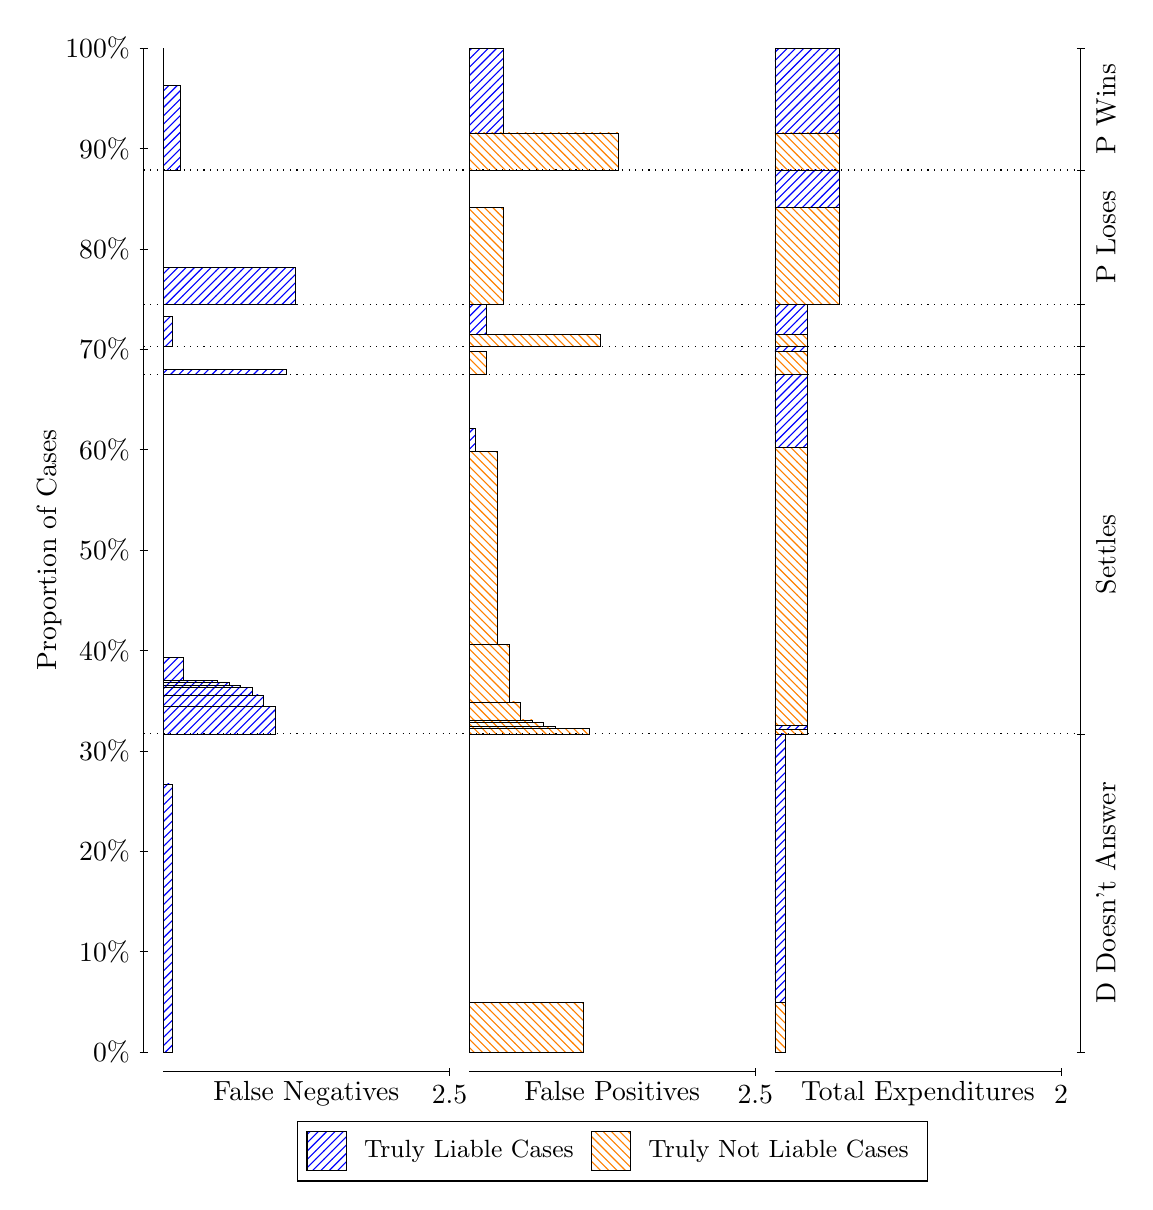
\begin{tikzpicture}
\draw[black, very thin] (1.5,1.75) -- (1.5,14.5);
\node[rotate=90, text=black, anchor=center] at (0.3, 8.125) {Proportion of Cases};
\draw[black, very thin] (1.45,1.75) -- (1.55,1.75);
\node[text=black, anchor=east] at (1.45, 1.75) {0\%};
\draw[black, very thin] (1.45,3.025) -- (1.55,3.025);
\node[text=black, anchor=east] at (1.45, 3.025) {10\%};
\draw[black, very thin] (1.45,4.3) -- (1.55,4.3);
\node[text=black, anchor=east] at (1.45, 4.3) {20\%};
\draw[black, very thin] (1.45,5.575) -- (1.55,5.575);
\node[text=black, anchor=east] at (1.45, 5.575) {30\%};
\draw[black, very thin] (1.45,6.85) -- (1.55,6.85);
\node[text=black, anchor=east] at (1.45, 6.85) {40\%};
\draw[black, very thin] (1.45,8.125) -- (1.55,8.125);
\node[text=black, anchor=east] at (1.45, 8.125) {50\%};
\draw[black, very thin] (1.45,9.4) -- (1.55,9.4);
\node[text=black, anchor=east] at (1.45, 9.4) {60\%};
\draw[black, very thin] (1.45,10.675) -- (1.55,10.675);
\node[text=black, anchor=east] at (1.45, 10.675) {70\%};
\draw[black, very thin] (1.45,11.95) -- (1.55,11.95);
\node[text=black, anchor=east] at (1.45, 11.95) {80\%};
\draw[black, very thin] (1.45,13.225) -- (1.55,13.225);
\node[text=black, anchor=east] at (1.45, 13.225) {90\%};
\draw[black, very thin] (1.45,14.5) -- (1.55,14.5);
\node[text=black, anchor=east] at (1.45, 14.5) {100\%};

\draw[black, very thin] (13.4,1.75) -- (13.4,14.5);
\draw[black, very thin] (13.35,1.75) -- (13.45,1.75);
\node[anchor=west] at (13.35, 1.75) {};
\draw[black, very thin] (13.35,5.7901) -- (13.45,5.7901);
\node[anchor=west] at (13.35, 5.7901) {};
\draw[black, very thin] (13.35,10.354) -- (13.45,10.354);
\node[anchor=west] at (13.35, 10.354) {};
\draw[black, very thin] (13.35,10.711) -- (13.45,10.711);
\node[anchor=west] at (13.35, 10.711) {};
\draw[black, very thin] (13.35,11.244) -- (13.45,11.244);
\node[anchor=west] at (13.35, 11.244) {};
\draw[black, very thin] (13.35,12.951) -- (13.45,12.951);
\node[anchor=west] at (13.35, 12.951) {};
\draw[black, very thin] (13.35,14.5) -- (13.45,14.5);
\node[anchor=west] at (13.35, 14.5) {};

\draw[black, very thin, pattern color=blue, pattern=north east lines] (1.75,1.75) rectangle (1.859,5.1556);
\draw[black, very thin, pattern color=orange, pattern=north west lines] (1.75,5.1556) rectangle (1.75,5.7901);
\draw[black, very thin, pattern color=blue, pattern=north east lines] (1.75,5.7901) rectangle (3.167,6.1425);
\draw[black, very thin, pattern color=blue, pattern=north east lines] (1.75,6.1425) rectangle (3.0217,6.286);
\draw[black, very thin, pattern color=blue, pattern=north east lines] (1.75,6.286) rectangle (2.8763,6.382);
\draw[black, very thin, pattern color=blue, pattern=north east lines] (1.75,6.382) rectangle (2.731,6.4066);
\draw[black, very thin, pattern color=blue, pattern=north east lines] (1.75,6.4066) rectangle (2.5857,6.4428);
\draw[black, very thin, pattern color=blue, pattern=north east lines] (1.75,6.4428) rectangle (2.4403,6.4667);
\draw[black, very thin, pattern color=blue, pattern=north east lines] (1.75,6.4667) rectangle (2.295,6.4694);
\draw[black, very thin, pattern color=blue, pattern=north east lines] (1.75,6.4694) rectangle (2.1497,6.4716);
\draw[black, very thin, pattern color=blue, pattern=north east lines] (1.75,6.4716) rectangle (2.0043,6.7625);
\draw[black, very thin, pattern color=orange, pattern=north west lines] (1.75,6.7625) rectangle (1.75,10.354);
\draw[black, very thin, pattern color=blue, pattern=north east lines] (1.75,10.354) rectangle (3.3123,10.417);
\draw[black, very thin, pattern color=orange, pattern=north west lines] (1.75,10.417) rectangle (1.75,10.711);
\draw[black, very thin, pattern color=blue, pattern=north east lines] (1.75,10.711) rectangle (1.859,11.095);
\draw[black, very thin, pattern color=orange, pattern=north west lines] (1.75,11.095) rectangle (1.75,11.244);
\draw[black, very thin, pattern color=blue, pattern=north east lines] (1.75,11.244) rectangle (3.4213,11.717);
\draw[black, very thin, pattern color=orange, pattern=north west lines] (1.75,11.717) rectangle (1.75,12.951);
\draw[black, very thin, pattern color=blue, pattern=north east lines] (1.75,12.951) rectangle (1.968,14.028);
\draw[black, very thin, pattern color=orange, pattern=north west lines] (1.75,14.028) rectangle (1.75,14.5);
\draw[black, very thin, pattern color=orange, pattern=north west lines] (5.6333,1.75) rectangle (7.0867,2.3844);
\draw[black, very thin, pattern color=blue, pattern=north east lines] (5.6333,2.3844) rectangle (5.6333,5.7901);
\draw[black, very thin, pattern color=orange, pattern=north west lines] (5.6333,5.7901) rectangle (7.1593,5.8591);
\draw[black, very thin, pattern color=orange, pattern=north west lines] (5.6333,5.8591) rectangle (7.014,5.8609);
\draw[black, very thin, pattern color=orange, pattern=north west lines] (5.6333,5.8609) rectangle (6.8687,5.8633);
\draw[black, very thin, pattern color=orange, pattern=north west lines] (5.6333,5.8633) rectangle (6.7233,5.8813);
\draw[black, very thin, pattern color=orange, pattern=north west lines] (5.6333,5.8813) rectangle (6.578,5.9312);
\draw[black, very thin, pattern color=orange, pattern=north west lines] (5.6333,5.9312) rectangle (6.4327,5.9416);
\draw[black, very thin, pattern color=orange, pattern=north west lines] (5.6333,5.9416) rectangle (6.4327,5.9669);
\draw[black, very thin, pattern color=orange, pattern=north west lines] (5.6333,5.9669) rectangle (6.2873,6.1971);
\draw[black, very thin, pattern color=orange, pattern=north west lines] (5.6333,6.1971) rectangle (6.142,6.9245);
\draw[black, very thin, pattern color=orange, pattern=north west lines] (5.6333,6.9245) rectangle (5.9967,9.3813);
\draw[black, very thin, pattern color=blue, pattern=north east lines] (5.6333,9.3813) rectangle (5.706,9.6722);
\draw[black, very thin, pattern color=blue, pattern=north east lines] (5.6333,9.6722) rectangle (5.6333,10.354);
\draw[black, very thin, pattern color=orange, pattern=north west lines] (5.6333,10.354) rectangle (5.8513,10.648);
\draw[black, very thin, pattern color=blue, pattern=north east lines] (5.6333,10.648) rectangle (5.6333,10.711);
\draw[black, very thin, pattern color=orange, pattern=north west lines] (5.6333,10.711) rectangle (7.3047,10.86);
\draw[black, very thin, pattern color=blue, pattern=north east lines] (5.6333,10.86) rectangle (5.8513,11.244);
\draw[black, very thin, pattern color=orange, pattern=north west lines] (5.6333,11.244) rectangle (6.0693,12.478);
\draw[black, very thin, pattern color=blue, pattern=north east lines] (5.6333,12.478) rectangle (5.6333,12.951);
\draw[black, very thin, pattern color=orange, pattern=north west lines] (5.6333,12.951) rectangle (7.5227,13.423);
\draw[black, very thin, pattern color=blue, pattern=north east lines] (5.6333,13.423) rectangle (6.0693,14.5);
\draw[black, very thin, pattern color=orange, pattern=north west lines] (9.5167,1.75) rectangle (9.6529,2.3844);
\draw[black, very thin, pattern color=blue, pattern=north east lines] (9.5167,2.3844) rectangle (9.6529,5.7901);
\draw[black, very thin, pattern color=orange, pattern=north west lines] (9.5167,5.7901) rectangle (9.9254,5.8504);
\draw[black, very thin, pattern color=blue, pattern=north east lines] (9.5167,5.8504) rectangle (9.9254,5.8983);
\draw[black, very thin, pattern color=orange, pattern=north west lines] (9.5167,5.8983) rectangle (9.9254,9.4292);
\draw[black, very thin, pattern color=blue, pattern=north east lines] (9.5167,9.4292) rectangle (9.9254,10.354);
\draw[black, very thin, pattern color=orange, pattern=north west lines] (9.5167,10.354) rectangle (9.9254,10.648);
\draw[black, very thin, pattern color=blue, pattern=north east lines] (9.5167,10.648) rectangle (9.9254,10.711);
\draw[black, very thin, pattern color=orange, pattern=north west lines] (9.5167,10.711) rectangle (9.9254,10.86);
\draw[black, very thin, pattern color=blue, pattern=north east lines] (9.5167,10.86) rectangle (9.9254,11.244);
\draw[black, very thin, pattern color=orange, pattern=north west lines] (9.5167,11.244) rectangle (10.334,12.478);
\draw[black, very thin, pattern color=blue, pattern=north east lines] (9.5167,12.478) rectangle (10.334,12.951);
\draw[black, very thin, pattern color=orange, pattern=north west lines] (9.5167,12.951) rectangle (10.334,13.423);
\draw[black, very thin, pattern color=blue, pattern=north east lines] (9.5167,13.423) rectangle (10.334,14.5);
\draw[black, dotted] (1.5,5.7901) -- (13.4,5.7901);
\draw[black, dotted] (1.5,10.354) -- (13.4,10.354);
\draw[black, dotted] (1.5,10.711) -- (13.4,10.711);
\draw[black, dotted] (1.5,11.244) -- (13.4,11.244);
\draw[black, dotted] (1.5,12.951) -- (13.4,12.951);
\draw[black, very thin] (1.75,1.5) -- (5.3833,1.5);
\node[text=black, anchor=north] at (3.5667, 1.5) {False Negatives};
\draw[black, very thin] (5.3833,1.45) -- (5.3833,1.55);
\node[text=black, anchor=north] at (5.3833, 1.45) {2.5};

\draw[black, very thin] (5.6333,1.5) -- (9.2667,1.5);
\node[text=black, anchor=north] at (7.45, 1.5) {False Positives};
\draw[black, very thin] (9.2667,1.45) -- (9.2667,1.55);
\node[text=black, anchor=north] at (9.2667, 1.45) {2.5};

\draw[black, very thin] (9.5167,1.5) -- (13.15,1.5);
\node[text=black, anchor=north] at (11.333, 1.5) {Total Expenditures};
\draw[black, very thin] (13.15,1.45) -- (13.15,1.55);
\node[text=black, anchor=north] at (13.15, 1.45) {2};

\node[text=black, centered, rotate=90] at (13.72, 3.77) {D Doesn't Answer};
\node[text=black, centered, rotate=90] at (13.72, 8.0719) {Settles};


\node[text=black, centered, rotate=90] at (13.72, 12.098) {P Loses};
\node[text=black, centered, rotate=90] at (13.72, 13.725) {P Wins};

\draw (7.449999999999999,1.5) node[draw=none] (baseCoordinate) {};
\begin{scope}[align=center]
        \matrix[scale=0.5, draw=black, below=0.5cm of baseCoordinate, nodes={draw}, column sep=0.1cm]{
            \node[rectangle, draw, minimum width=0.5cm, minimum height=0.5cm, pattern color=blue, pattern=north east lines] {}; &
            \node[draw=none, font=\small, text=black] (B) {Truly Liable Cases}; &
            \node[rectangle, draw, minimum width=0.5cm, minimum height=0.5cm, pattern color=orange, pattern=north west lines] {}; &
            \node[draw=none, font=\small, text=black] (B) {Truly Not Liable Cases}; \\
            };
\end{scope}

\end{tikzpicture}
\end{document}